\documentclass{beamer}

\usepackage{graphicx}
\usepackage{caption}

\begin{document}
	
	\begin{frame}[plain]
		\begin{figure}
			\centering
			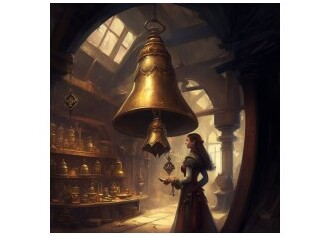
\includegraphics[width=\textwidth,height=0.85\textheight,keepaspectratio]{61.jpg}
			\caption{Inside a steampunk shop, with a large metallic bell}
		\end{figure}
	\end{frame}
	
	\begin{frame}[plain]
		\begin{figure}
			\centering
			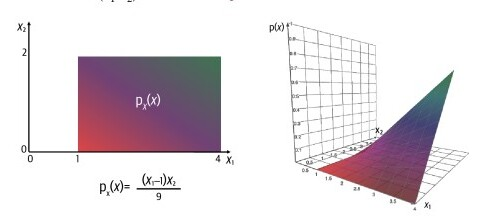
\includegraphics[width=\textwidth,height=0.85\textheight,keepaspectratio]{62.jpg}
			\caption{A probability distribution pX x defined over two dimensions, shown in 2D
				(left) and 3D (right)}
		\end{figure}
	\end{frame}
	
	\begin{frame}[plain]
		\begin{figure}
			\centering
			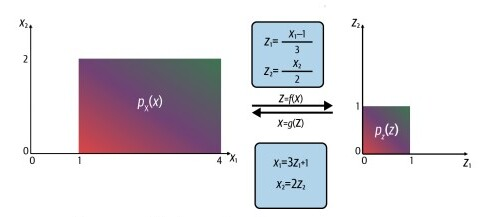
\includegraphics[width=\textwidth,height=0.85\textheight,keepaspectratio]{63.jpg}
			\caption{Changing variables between X and Z}
		\end{figure}
	\end{frame}
	
	\begin{frame}[plain]
		\begin{figure}
			\centering
			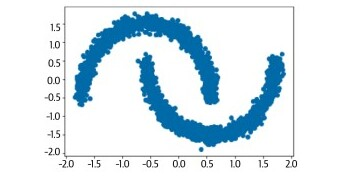
\includegraphics[width=\textwidth,height=0.85\textheight,keepaspectratio]{64.jpg}
			\caption{The two moons dataset in two dimensions}
		\end{figure}
	\end{frame}
	
	\begin{frame}[plain]
		\begin{figure}
			\centering
			
\includegraphics[width=\textwidth,height=0.85\textheight,keepaspectratio]{65.jpg}
			\caption{A coupling layer outputs two tensors that are the same shape as the input: a
				scaling factor (s) and a translation factor (t)}
		\end{figure}
	\end{frame}
	
	\begin{frame}[plain]
		\begin{figure}
			\centering
			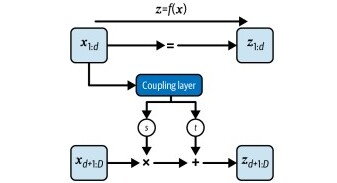
\includegraphics[width=\textwidth,height=0.85\textheight,keepaspectratio]{66.jpg}
			\caption{The process of transforming the input x through a coupling layer}
		\end{figure}
	\end{frame}
	
	\begin{frame}[plain]
		\begin{figure}
			\centering
			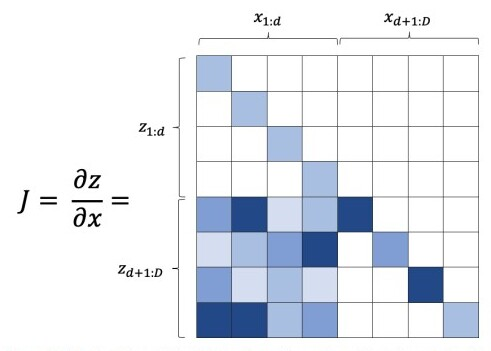
\includegraphics[width=\textwidth,height=0.85\textheight,keepaspectratio]{67.jpg}
			\caption{The Jacobian matrix of the transformation—a lower triangular matrix, with
				determinant equal to the product of the elements along the diagonal}
		\end{figure}
	\end{frame}
	
	\begin{frame}[plain]
		\begin{figure}
			\centering
			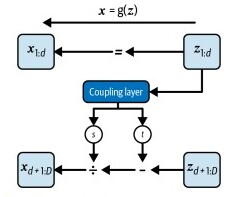
\includegraphics[width=\textwidth,height=0.85\textheight,keepaspectratio]{68.jpg}
			\caption{The inverse function x = g(z)}
		\end{figure}
	\end{frame}
	
	\begin{frame}[plain]
		\begin{figure}
			\centering
			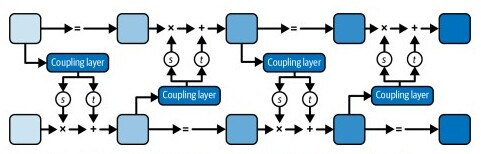
\includegraphics[width=\textwidth,height=0.85\textheight,keepaspectratio]{69.jpg}
			\caption{Stacking coupling layers, alternating the masking with each layer}
		\end{figure}
	\end{frame}
	
	\begin{frame}[plain]
		\begin{figure}
			\centering
			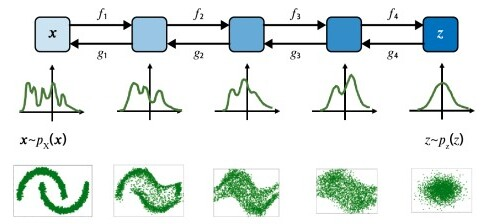
\includegraphics[width=\textwidth,height=0.85\textheight,keepaspectratio]{610.jpg}
			\caption{Transforming between the complex distribution pX(x) and a simple Gaus‐
				sian pZ(z) in 1D (middle row) and 2D (bottom row)}
		\end{figure}
	\end{frame}
	
	\begin{frame}[plain]
		\begin{figure}
			\centering
			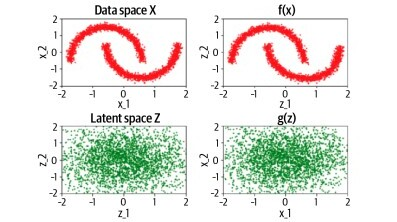
\includegraphics[width=\textwidth,height=0.85\textheight,keepaspectratio]{611.jpg}
			\caption{The RealNVP model inputs (left) and outputs (right) before training, for the
				forward process (top) and the reverse process (bottom)}
		\end{figure}
	\end{frame}
	
	\begin{frame}[plain]
		\begin{figure}
			\centering
			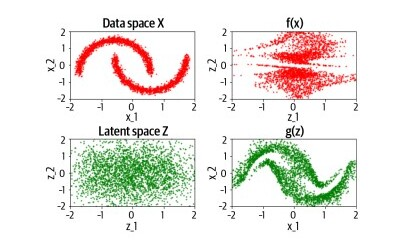
\includegraphics[width=\textwidth,height=0.85\textheight,keepaspectratio]{612.jpg}
			\caption{The RealNVP model inputs (left) and outputs (right) after training, for the
				forward process (top) and the reverse process (bottom)}
		\end{figure}
	\end{frame}
	
	\begin{frame}[plain]
		\begin{figure}
			\centering
			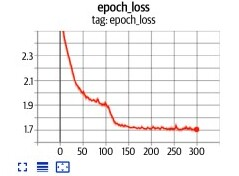
\includegraphics[width=\textwidth,height=0.85\textheight,keepaspectratio]{613.jpg}
			\caption{The loss curve for the RealNVP training process}
		\end{figure}
	\end{frame}
	
	\begin{frame}[plain]
		\begin{figure}
			\centering
			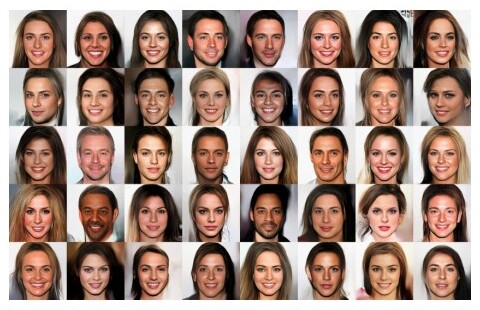
\includegraphics[width=\textwidth,height=0.85\textheight,keepaspectratio]{614.jpg}
			\caption{Random samples from the GLOW model}
		\end{figure}
	\end{frame}
	
	\begin{frame}[plain]
		\begin{figure}
			\centering
			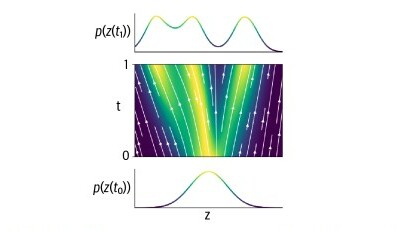
\includegraphics[width=\textwidth,height=0.85\textheight,keepaspectratio]{615.jpg}
			\caption{FFJORD models the transformation between the data distribution and a
				standard Gaussian via an ordinary differential equation, parameterized by a neural
				network}
		\end{figure}
	\end{frame}
	
\end{document}